\documentclass[c]{beamer}
\usepackage[latin1]{inputenc}
\usepackage{amsmath}
\usepackage{amssymb}
\usepackage{graphics}
\usepackage{nicefrac}
\usepackage{amsthm}

\usetheme{Warsaw}

\title{A gentle introduction to Complexity Theory}
\author{Matthias Kausl \\ Lukas Lang}

\institute{Vienna University of Technology}
\date{\today}
\begin{document}

\begin{frame}
\titlepage
\end{frame}

\begin{frame}{Outline}
	\tableofcontents
\end{frame}

\section{Motivation}

\begin{frame}{Motivation}
	% Why complexity analysis is needed.
	% Table with growth of functions. Input/Runtime.
          
	\begin{block}{A blue block}
		some text.
          \end{block}
\end{frame}

\section{Models of Computation}
\begin{frame}{Models of Computation (or why it doesn't matter)}
          % Register machines, partial recursive functions, Turing machine or just source code.
          % Church-Turing thesis.
          \begin{itemize}
			\item Which Models of Computation to use?
			\item formal (deterministic) models:
			\begin{itemize}
				\item Lambda calculus
				\item Register machines
				\item Turing machines
				\item ... many more
			\end{itemize}
			\item "real" computers: many different architectures...
		  \end{itemize}
\end{frame}		

\begin{frame}{Models of Computation (or why it doesn't matter)}  
Turing Machine

 \begin{itemize}
			\item one tape with infinite amount of memory cells.
			\item a head reading/writing on the tape one cell at a time.
			\item an action table.
			\item a state register.
 \end{itemize}
 
\begin{center}
 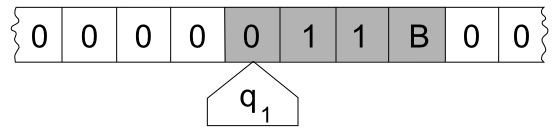
\includegraphics[scale=0.3]{images/tm.png} 
\end{center}
\end{frame}	

\begin{frame}{Models of Computation (or why it doesn't matter)}  
	\begin{block}{ Church-Turing thesis }
		All computable functions are computable by a Turing machine.
    \end{block}
    \begin{block}{ Strong Church-Turing thesis }
		All models of computation can be simulated by a Turing machine with at most polynomial more time/space.
    \end{block}
\end{frame}

\section{Computational Problems}
\begin{frame}{Problems}
          % What is a problem (infinite number of instances and a question).
          % Some easy examples (maybe basic logic or graph problems).
         For a computational problem, we are interested in
         \begin{itemize}
			\item the best (in terms of space/time) algorithm solving the problem.
			\item a proof that it there is no better algorithm.
		\end{itemize}	  
	
\end{frame}

\begin{frame}{Problems}
        What is a \textbf{problem}?
         \begin{itemize}
			\item an infinite number of inputs ("instance").
			\item a question.
		\end{itemize}	 
		
		If the question is a yes/no question: \textbf{decision problem}. 		
	
\end{frame}

\begin{frame}{Problems - Examples}
    \begin{block}{ HALTING }
		Input: A \textbf{computer program} and an \textbf{input string}.\\
		Question: Does the computer program terminate on that input string?
    \end{block}	
	
	\begin{block}{ REACHABILITY }
		Input: A graph $G$ and two nodes $s,t$\\
		Question: Is $t$ reachable from $s$?
    \end{block}	
    
    \begin{block}{ PRIMES }
		Input: An integer $P$\\
		Question: Is $P$ a prime number?
    \end{block}	
    
\end{frame}

\section{Complexity Classes}
\begin{frame}{Complexity}
          % How to capture complexity. Bit complexity.
          % Time/Space complexity. Polynomial/Exponential.
          % Maybe state a short example algorithm and complexity.
      What is the complexity of \textbf{PRIMES} ?
	 \begin{itemize}
			\item Time complexity: computation steps needed to answer the question.
			\item Space complexity: how much memory do we need?
	 \end{itemize}
	 
	 \textbf{PRIMES} can be solved in polynomial time in the size of the input (AKS primality test).
	 
\end{frame}

\begin{frame}{Complexity Classes}
	% What are natural classes? Give examples + problems.
	% P=NP question (can we efficiently solve all problems where we can check the solution efficiently?)
	% 1 million dollar question (and a few more)
	% Simpsons and futurama picture.
    Classify problems according to their time and space complexity.
	\begin{block}{PTIME (or simply P)}
		Problems that can be decided by a deterministic Turing machine in polynomial time in the size of the input.
    \end{block}
    Examples: \textbf{Prime, Reachability}
    \begin{block}{NP (non-deterministic polynomial time)}
		Problems that can be decided by a \textbf{non-deterministic} Turing machine in time polynomial in the size of the input.
    \end{block}
    Examples: \textbf{Integer Factorization, SAT, Travelling Salesman Problem}
\end{frame}

\begin{frame}{Complexity Classes}
    \begin{block}{PSPACE}
		Problems that can be decided by a deterministic Turing machine in polynomial \textbf{space} in the size of the input.
    \end{block}
    \begin{block}{EXPTIME (or simply EXP)}
		Problems that can be decided by a deterministic Turing machine in exponential \textbf{time} in the size of the input.
    \end{block}
\end{frame}

\begin{frame}{Complexity Classes}
 
 \begin{block}{Big question in computer science}
 	$P\stackrel{?}{=}NP$, i.e. can we efficiently solve all problems where we can check the solution efficiently?
 \end{block}
 e.g. checking whether $3*5 = 15$ is easy but the other way is hard.

 \medskip
 The Clay Mathematics Institute offers a 1 million dollar prize for a solution!
 
 We know that $ P \subseteq NP$ but not the converse. 
\end{frame}

\section{Quantum Complexity}

\begin{frame}{Quantum Complexity}

Where do quantum computers fit in?

new computational model to analyse quantum complexity:
\begin{itemize}
\item Quantum Turing machine
\item Quantum circuits
\end{itemize}

\end{frame}

\begin{frame}{Quantum Turing Machine}

A Quantum Turing Machine is represented by $|x;n;m>$
\begin{itemize}
\item slots on the tape are an infinite number of qbits: $m_i$ where $i \in Z$ 
\item states are represented by a finite number of qbits: $n_i$ where $i \in Z$
\item $x$ representing the position on a tape
\item one computation step is a transition $|\psi(n)> = U|\psi(n-1)>$ where
U is a reversible, unitary operator

\end{itemize}

\end{frame}

\begin{frame}{Quantum Turing Machine}

further conditions on U reflect the usual restrictions on turing machines: 
\begin{itemize}
\item one qbit at a time is manipulated
\item the tape position cannot change by more than one unit
\item a QTM halts if two consecutive states are identical 
\end{itemize}
\medskip
\begin{footnotesize}
details : Deutsch, David (July 1985). "Quantum theory, the Church-Turing principle and the universal quantum computer"
\url{http://www.ceid.upatras.gr/tech_news/papers/quantum_theory.pdf}
\end{footnotesize}

\end{frame}

\begin{frame}{Quantum Gates}
\begin{itemize}
\item one unitary transformation U represented in a quantum gate
\item universality: CNOT and singe qbit gates
\item one computation step: ??
\end{itemize}
\end{frame}

% Non-deterministic and randomized computation.
% Common misconceptions:
% - Factoring: consider bit complexity and not value complexity (otherwise O(n^2) algorithm would be easy).
% - Quantum computers solve NP-hard problems.
% - Quantum computers break cryptography.

\begin{frame}{Common misconceptions}
\begin{itemize}
\item Quantum computers solve NP-hard problems? \\
$\Rightarrow$ we don't know yet.
\item Quantum computers break cryptography? \\
\begin{itemize}
\item Shor's algorithm can factorize integers in polynomial time.
\item but there might also be a classical algorithm.
\item also: many Qubits needed.
\end{itemize}
\end{itemize}
\end{frame}

\begin{frame}{The class BQP}
	\begin{block}{BQP}
		BQP (bounded error quantum polynomial time) is the class of decision problems solvable by a quantum computer in polynomial time, with an error probability of at most 1/3 for all instances.
	\end{block}
	http://en.wikipedia.org/wiki/BQP
\end{frame}

\begin{frame}{The class BQP}
	\begin{block}{Elementary quantum operations (or quantum gates)}
		A quantum operation is \emph{elementary}, or sometimes a \emph{quantum gate}, if it acts on three or less qubits of the register.\footnote{The constant 3 is arbitrary!}
	\end{block}
	
	\begin{block}{Quantum computation and BQP}
		A function $f:\{0,1\}^{*} \rightarrow \{0,1\}$ is \emph{computable in quantum $T(n)$-time} if there is a polynomial-time classical TM that takes some input and outputs the description of quantum gates such that for every $x \in \{0,1\}^{n}$ we can compute $f(x)$ by applying the quantum operations with probability $\ge \nicefrac{2}{3}$. A function $f$ is in BQP if there is some polynomial $p$ s.t. $f$ is computable in quantum $p(n)$-time.
	\end{block}
\end{frame}


\begin{frame}{The class BQP}

\begin{center}
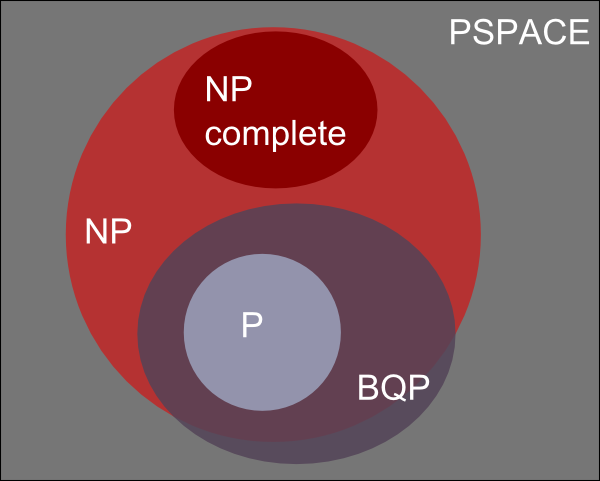
\includegraphics[scale=0.20]{images/classes.png} 	
\end{center}

\begin{itemize}
\item $\mbox{P} \subseteq \mbox{NP}  \subseteq \mbox{PSPACE} \subseteq \mbox{EXPTIME} $

\item $\mbox{P} \subsetneq \mbox{EXPTIME}$
	\end{itemize}
	
\end{frame}

\begin{frame}{Conclusion}

	
	
\end{frame}

\end{document}